\section{Introducción}

\subsection{Especificaciones iniciales del sistema a diseñar y construir}

El proyecto consiste en el desarrollo de un sistema de procesamiento de audio en tiempo real con un sistema centrado en un microprocesador.

El sistema permitirá entrada de audio a través de un módulo de radio FM y la lectura de canciones de una tarjeta microSD externa. Tras capturar dicho audio, se le aplicará un procesamiento digital implementado mediante la librería CMSIS DSP y se reproducirá por un altavoz o unos auriculares.

La interacción con el sistema se realizará a través de una pantalla táctil o una interfaz web, la cual requiere conexión a través de Ethernet. Dicha interfaz permite seleccionar la entrada de audio, controlar el volumen y ecualización de audio y elegir la salida. Además, permite controlar la emisora de radio sintonizada.

El sistema almacenará los parámetros seleccionados (entrada, salida y filtros) y una lista de emisoras favoritas en la tarjeta microSD, los cuales se cargarán al iniciar el equipo.

El sistema será completamente autónomo, contando con una batería con su correspondiente circuitería de carga, protección y medición de consumo. Se ofrecerá información sobre la batería en la interfaz gráfica del sistema. Además, el sistema contará con un modo de bajo consumo para alargar la duración de dicha batería.

Para la selección de canciones se permitirá el uso de tarjetas NFC preconfiguradas con canciones o emisoras preconfiguradas, para la interacción sin interfaz gráfica. Por último, el sistema utilizará el RTC integrado en la placa para mantener la hora y el protocolo SNTP para la sincronización.

\subsection{Especificaciones finales del sistema diseñado y construido}

El sistema permite la entrada de audio a través del Sintonizador FM y la lectura de canciones de una tarjeta microSD externa  mediante un reproductor MP3. Tras capturar dicho audio, se le aplica el procesamiento digital implementado mediante la librería CMSIS DSP y se reproduce por un altavoz o unos auriculares.

La interacción con el sistema se realiza a través de la pantalla táctil o mediante la interfaz web, la cual requiere conexión a través de Ethernet. Dicha interfaz nos permite seleccionar la entrada de audio, controlar el volumen y aplicar la ecualización deseada al audio y elegir la salida. Además, permite seleccionar y controlar la emisora de radio sintonizada.

El sistema permite la lectura de los parámetros de configuración seleccionados (entrada, salida, filtros y volumen) y una lista de canciones de la tarjeta uSD, escritos mediante un ordenador.

Por otra parte, el sistema permite almacenar un mapa de frecuencia a emisora en el almacenamiento de la propia tarjeta.

El sistema no es completamente autónomo,ya que, aunque cuente con una batería con su correspondiente circuitería de carga, protección y medición de consumo, el sistema necesita una conexión constante mediante el \texttt{ST\_Link}. Se ofrece información sobre el consumo medido en la interfaz gráfica del sistema. Además, el sistema cuenta con un modo de bajo consumo para alargar la duración de dicha batería.

Para la selección de canciones y emisoras, se permitirá el uso de tarjetas NFC preconfiguradas con canciones o emisoras preconfiguradas, para la interacción sin interfaz gráfica. Por último, el sistema utiliza el RTC integrado en la propia placa para mantener la hora y fecha actual mediante la sincronización son un servidor SNTP.

A continuación se adjunta una imagen del sistema completo, con todos su componentes y en su total funcionamiento:

\begin{figure}[!hp]
    \centering
    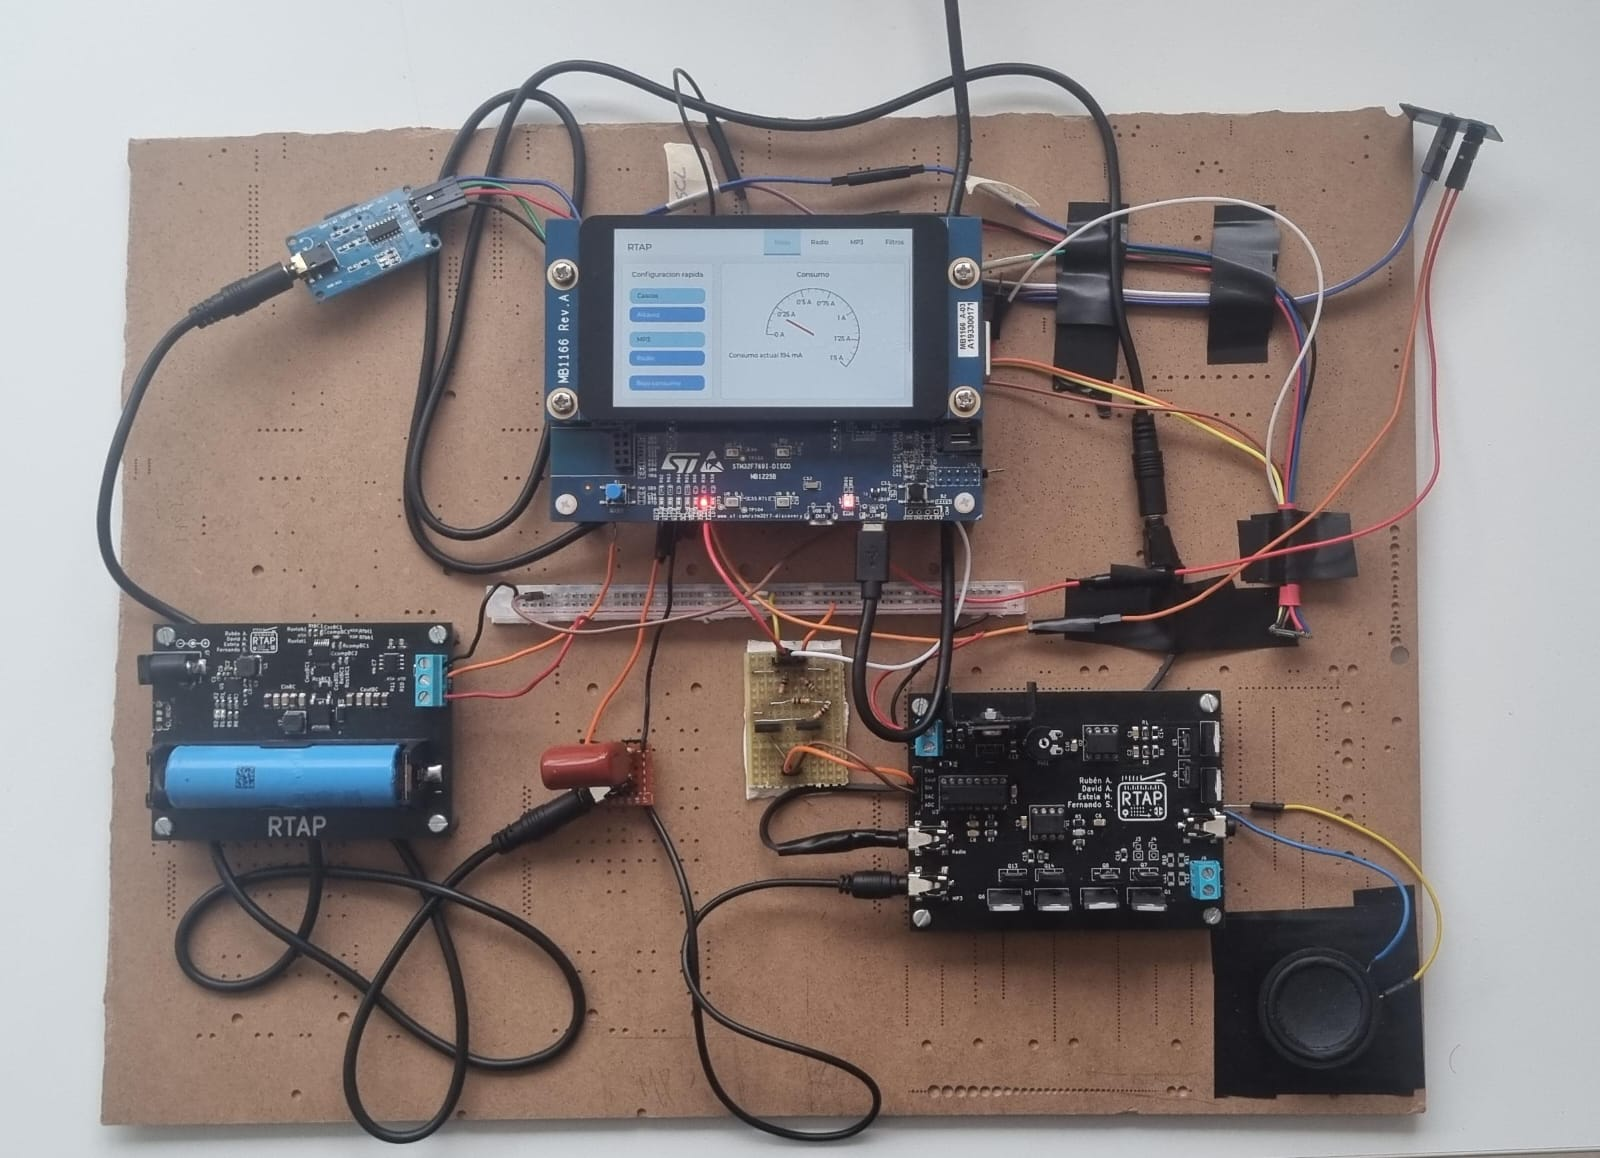
\includegraphics[width=\textwidth]{images/1/Foto_Sistema.jpg}
    \caption{Sistema Completo}
    \label{fig:1-Sistema_Completo}
\end{figure}